\documentclass[handout]{ximera}
%handout:  for handout version with no solutions or instructor notes
%handout,instructornotes:  for instructor version with just problems and notes, no solutions
%noinstructornotes:  shows only problem and solutions

%% handout
%% space
%% newpage
%% numbers
%% nooutcomes

%I added the commands here so that I would't have to keep looking them up
%\newcommand{\RR}{\mathbb R}
%\renewcommand{\d}{\,d}
%\newcommand{\dd}[2][]{\frac{d #1}{d #2}}
%\renewcommand{\l}{\ell}
%\newcommand{\ddx}{\frac{d}{dx}}
%\everymath{\displaystyle}
%\newcommand{\dfn}{\textbf}
%\newcommand{\eval}[1]{\bigg[ #1 \bigg]}

%\begin{image}
%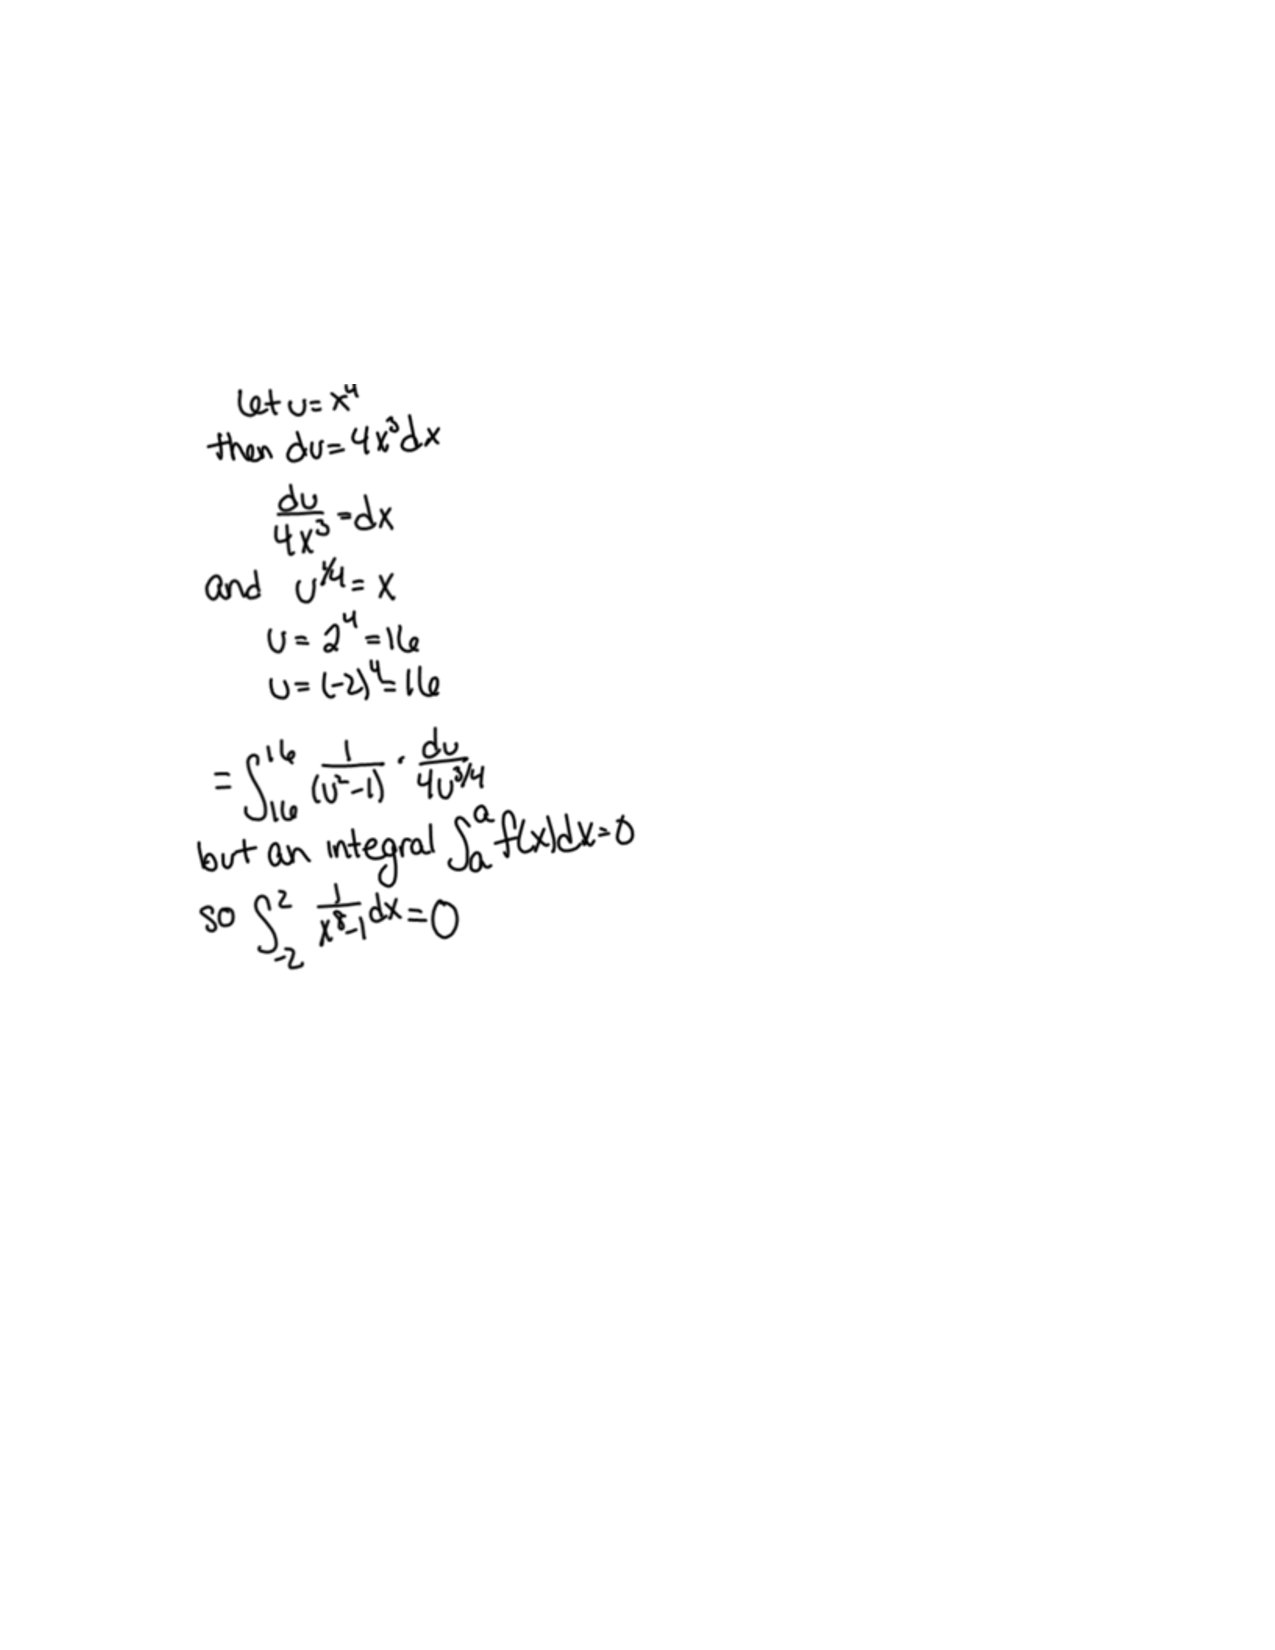
\includegraphics[trim= 170 420 250 180]{Figure1.pdf}
%\end{image}

%add a ``.'' below when used in a specific directory.
\newcommand{\RR}{\mathbb R}
\renewcommand{\d}{\,d}
\newcommand{\dd}[2][]{\frac{d #1}{d #2}}
\renewcommand{\l}{\ell}
\newcommand{\ddx}{\frac{d}{dx}}
\newcommand{\dfn}{\textbf}
\newcommand{\eval}[1]{\bigg[ #1 \bigg]}

\usepackage{multicol}

\renewenvironment{freeResponse}{
\ifhandout\setbox0\vbox\bgroup\else
\begin{trivlist}\item[\hskip \labelsep\bfseries Solution:\hspace{2ex}]
\fi}
{\ifhandout\egroup\else
\end{trivlist}
\fi} %% we can turn off input when making a master document

\title{Section 12.3: Dot Products}  

\begin{document}
\begin{abstract}		\end{abstract}
\maketitle


\section{Warm up:}

%problem1
\begin{problem}
If $\vec{u} = \hat{\imath} - 2 \hat{\jmath}$ and $\vec{v} = 3 \hat{\imath} + 4 \hat{k}$, find $\vec{u} \cdot \vec{v}$.
	\begin{freeResponse}
	Note that these vectors are in $\mathbb{R}^3$ and not $\mathbb{R}^2$.
	\[
	\vec{u} \cdot \vec{v} = (1 \cdot 3) + (-2 \cdot 0) + (0 \cdot 4) = \boxed{3}.
	\]
	\end{freeResponse}
	
\begin{instructorNotes}
Make sure that students realize that $\vec{u} = \langle 3,4,0 \rangle$ and not $\langle 3,4 \rangle$.
\end{instructorNotes}

\end{problem}






\section{Group work:}




%problem 2
\begin{problem}
Find a vector (in the $xy$-plane) with length $4$ that makes a $\frac{\pi}{3}$ radian angle with the vector $\langle 3,4 \rangle$.
	\begin{freeResponse}
	Let $\vec{v} = \langle a,b \rangle$ denote a vector that we are looking for, and let $\vec{u} = \langle 3,4 \rangle$.  
	First note that
		\[
		| \vec{u} | = \sqrt{9 + 16} = 5.
		\]
	So
		\[
		\vec{u} \cdot \vec{v} = | \vec{u} | | \vec{v} | \cos \left( \frac{\pi}{3} \right) = 5 \cdot 4 \cdot \frac{1}{2} = 10.
		\]
	Then we have the following two equations:
		\begin{align}
		&10 = \vec{u} \cdot \vec{v} = 3a + 4b  \label{eqn1}  \\
		&16 = | \vec{v} |^2 = a^2 + b^2  \label{eqn2}  .
		\end{align}
	Solving equation \eqref{eqn1} for $a$ gives us
		\[
		a = \frac{10 - 4b}{3}.
		\]
	Plugging this into equation \eqref{eqn2} yields
		\begin{align*}
		\left( \frac{10-4b}{3} \right)^2 + b^2 &= 16  \\
		(10-4b)^2 + 9b^2 &= 144  \\
		16b^2 -80b + 100 + 9b^2 &= 144  \\
		25b^2 - 80b - 44 &= 0
		\end{align*}
	Using the quadratic formula gives
		\begin{align*}
		b &= \frac{80 \pm \sqrt{(-80)^2 - 4(25)(-44)}}{2(25)}  \\
		&= \frac{80 \pm \sqrt{10800}}{50}  \\
		&= \frac{80 \pm 60\sqrt{3}}{50}  \\
		&= \frac{8 \pm 6\sqrt{3}}{5}.
		\end{align*}
		
	We can choose either value for $b$.  
	Choosing $b = \frac{8 + 6 \sqrt{3}}{5}$ gives a value of $a = \frac{10 - 4 \left( \frac{8+6\sqrt{3}}{5} \right)}{3}$.
	Thus,
		\[
		\vec{v} = \boxed{ \left\langle \frac{10 - 4 \left( \frac{8+6\sqrt{3}}{5} \right)}{3} ,  \frac{8 + 6 \sqrt{3}}{5} \right\rangle }
		\]
	\end{freeResponse}

\end{problem}

\begin{instructorNotes}
The students need to assimilate a lot of information in this problem.  
They need to ``name'' the unknown vector (say $\langle a, b \rangle$).  
Then, they need to realize that both $\langle 3,4 \rangle \cdot \langle 3,4 \rangle = 3a + 4b$ and that $\bigr| \langle 3,4 \rangle \bigr| \cdot \bigr| \langle a,b \rangle \bigr| \cos \left( \frac{\pi}{3} \right) = 5 \cdot 4 \cdot \frac{1}{2}$, giving $3a + 4b = 10$.  
Lastly, they also need to realize that $a^2 + b^2 = 16$.  
A picture illustrating that there could be two such vectors would be helpful.
\end{instructorNotes}








%problem 3
\begin{problem}
Answer the following questions about $\text{proj}_v u$.
	\begin{enumerate}
	\item  Is $\text{proj}_v u$ a vector of the form $c \vec{v}$ or $c \vec{u}$ (where $c$ is a real number)?  
	ie, is $\text{proj}_v u$ parallel to $\vec{u}$ or $\vec{v}$?  
	
	\item  If $\vec{u} = 5 \hat{\imath} + 6 \hat{\jmath} - 3 \hat{k}$ and $\vec{v} = 2 \hat{\imath} - 4 \hat{\jmath} + 4 \hat{k}$, find $\text{proj}_v u$.
	
	\item  For $\vec{u}$ and $\vec{v}$ from part (b), write $\vec{u}$ as the sum of two perpendicular vectors, one of which is parallel to $\vec{v}$.  Verify that the other vector is perpendicular to $\vec{v}$.
	\end{enumerate}
	
	\begin{freeResponse}
	\begin{enumerate}
	\item  $\boxed{c \vec{v}}$
	
	\item  
		\begin{align*}
		\text{proj}_v u 
		&= \frac{\vec{u} \cdot \vec{v}}{\vec{v} \cdot \vec{v}} \vec{v}  \\
		&= \frac{10-24-12}{4+16+16} \langle 2,-4,4 \rangle  \\
		&= \boxed{- \frac{13}{18} \langle 2,-4,4 \rangle  }
		\end{align*}
	
	
	
	\item  A schematic picture of the situation is as follows:
		\begin{image}
		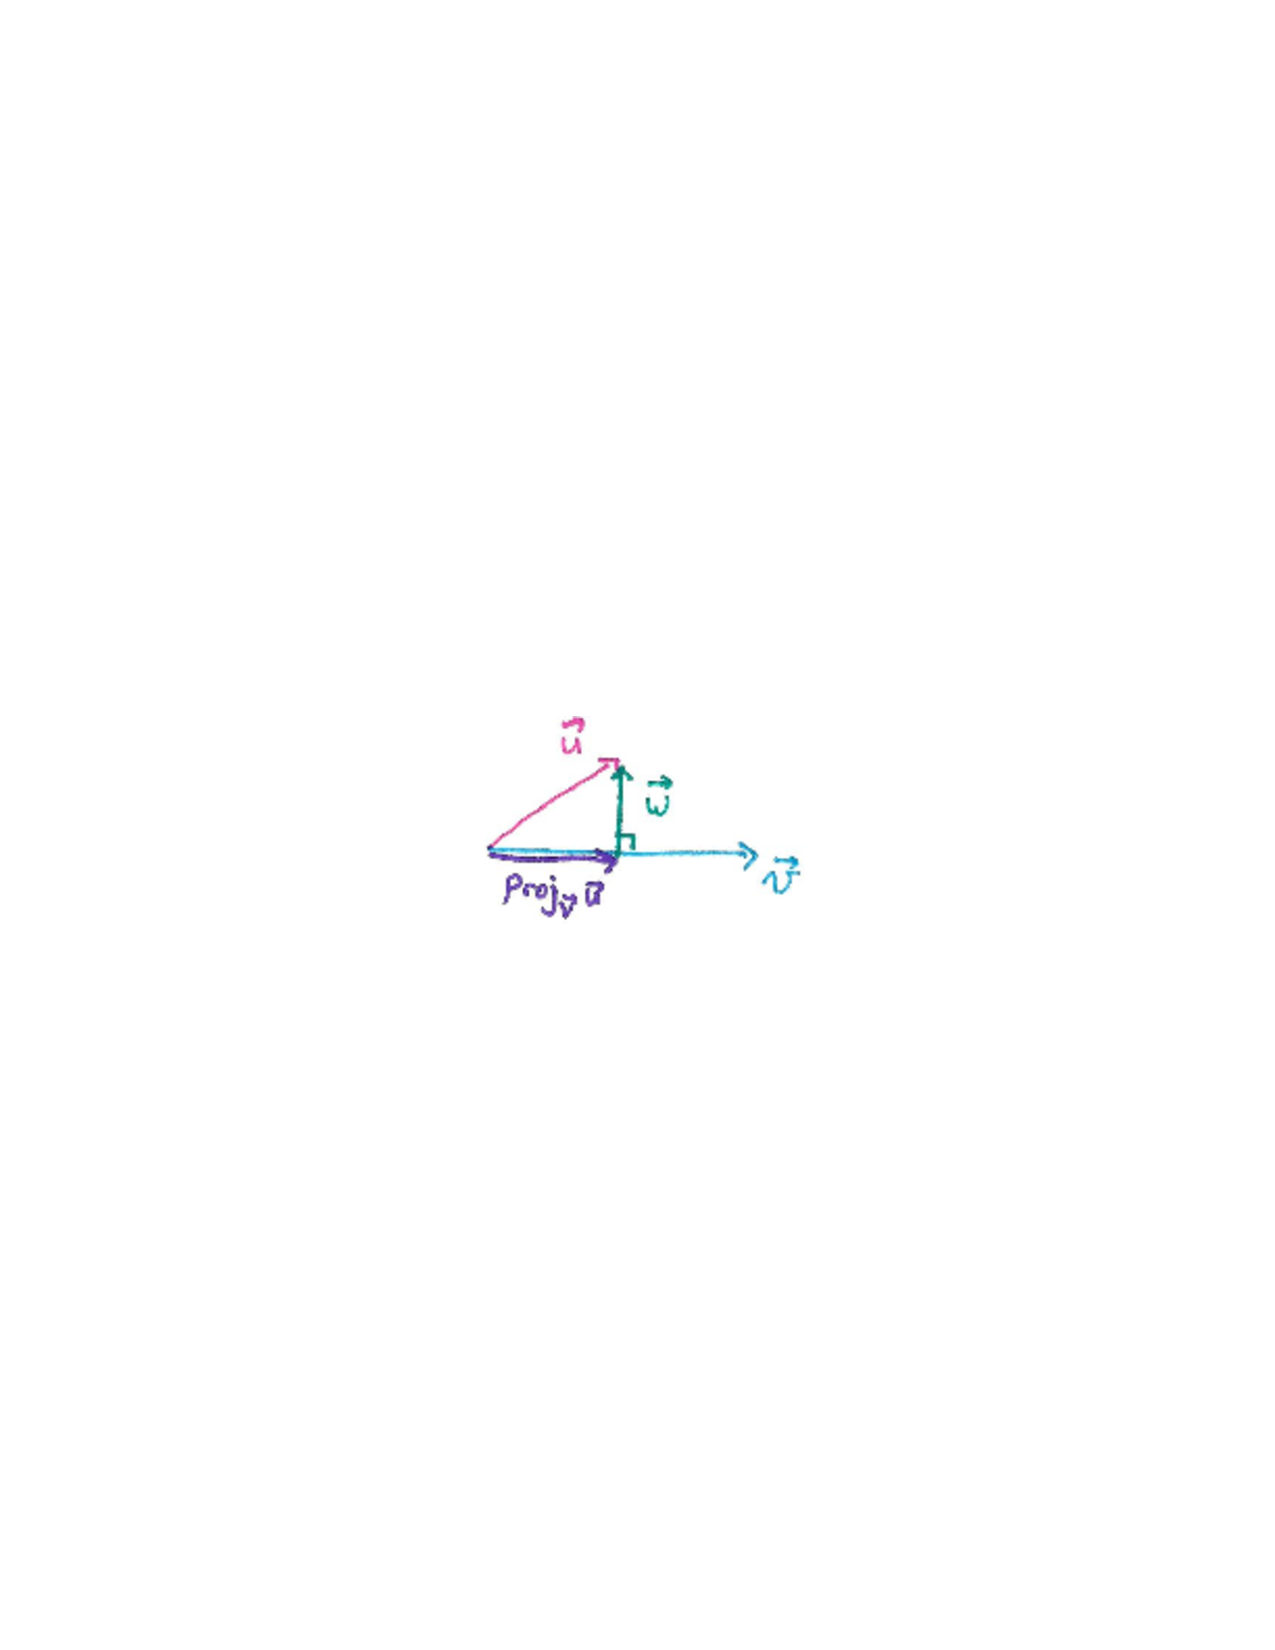
\includegraphics[trim= 170 350 170 350, scale=1]{Figure12-3-1.pdf}
		\end{image}
		
	The vector which is parallel to $\vec{v}$ is 
		\[
		\text{proj}_v u = \boxed{\left\langle - \frac{13}{9}, \frac{26}{9}, - \frac{26}{9} \right\rangle}
		\]
	The vector which is orthogonal to $\vec{v}$ is
		\begin{align*}
		\vec{w} := \vec{u} - \text{proj}_v u
		&= \left\langle 5,6,-3 \right\rangle - \left\langle - \frac{13}{9}, \frac{26}{9}, - \frac{26}{9} \right\rangle  \\
		&= \boxed{\left\langle \frac{58}{9}, \frac{28}{9}, - \frac{1}{9} \right\rangle}
		\end{align*}
	And, clearly, $\text{proj}_v u + \vec{w} = \text{proj}_v u + (\vec{u} - \text{proj}_v u) = \vec{u}$.  
	
	To verify that $\vec{w}$ is orthogonal to $\vec{v}$, we take the dot product and show we get 0. \\
	$\vec{w} \cdot \vec{v} = \left\langle \frac{58}{9}, \frac{28}{9}, - \frac{1}{9} \right\rangle \cdot \left\langle 2,4,4 \right\rangle  = \frac{58}{9} (2) + \frac{28}{9}  (-4) -  \frac{1}{9} (4) = \frac{116-112 -4}{9}=0$ 
	
	\end{enumerate}
	
	\end{freeResponse}

\end{problem}

\begin{instructorNotes}
Working with projections.
\end{instructorNotes}


%
%
%
%
%
%
%%problem 4
%\begin{problem}
%A $500kg$ lead hangs from three cables of equal length that are located at the points $(-2,0,0)$, $(1, \sqrt{3},0)$, and $(1, -\sqrt{3},0)$.  
%The load is located at $(0,0,-2 \sqrt{3})$.  
%Find the vectors describing the forces on the cables due to the load.
%	\begin{freeResponse}
%	Let $A = (1,-\sqrt{3},0)$, $B = (1, \sqrt{3},0)$, and $C = (-2,0,0)$, and let $M = (0,0, -2\sqrt{3})$.  
%	Let $\vec{a}$, $\vec{b}$, and $\vec{c}$ denote the vectors from $A$, $B$, and $C$ to $M$, respectively.  
%	ie, 
%		\begin{align*}
%		&\vec{a} = \langle 0-1, 0 - (-\sqrt{3}), -2 \sqrt{3}-0 \rangle = \langle -1, \sqrt{3}, -2 \sqrt{3} \rangle  \\
%		&\vec{b} = \langle 0-1, 0 - \sqrt{3}, -2 \sqrt{3} - 0 \rangle = \langle -1, -\sqrt{3}, -2 \sqrt{3} \rangle  \\
%		&\vec{c} = \langle 0- (-2), 0 - 0, -2 \sqrt{3} - 0 \rangle = \langle 2, 0, -2 \sqrt{3} \rangle .
%		\end{align*}
%		
%		\begin{image}
%		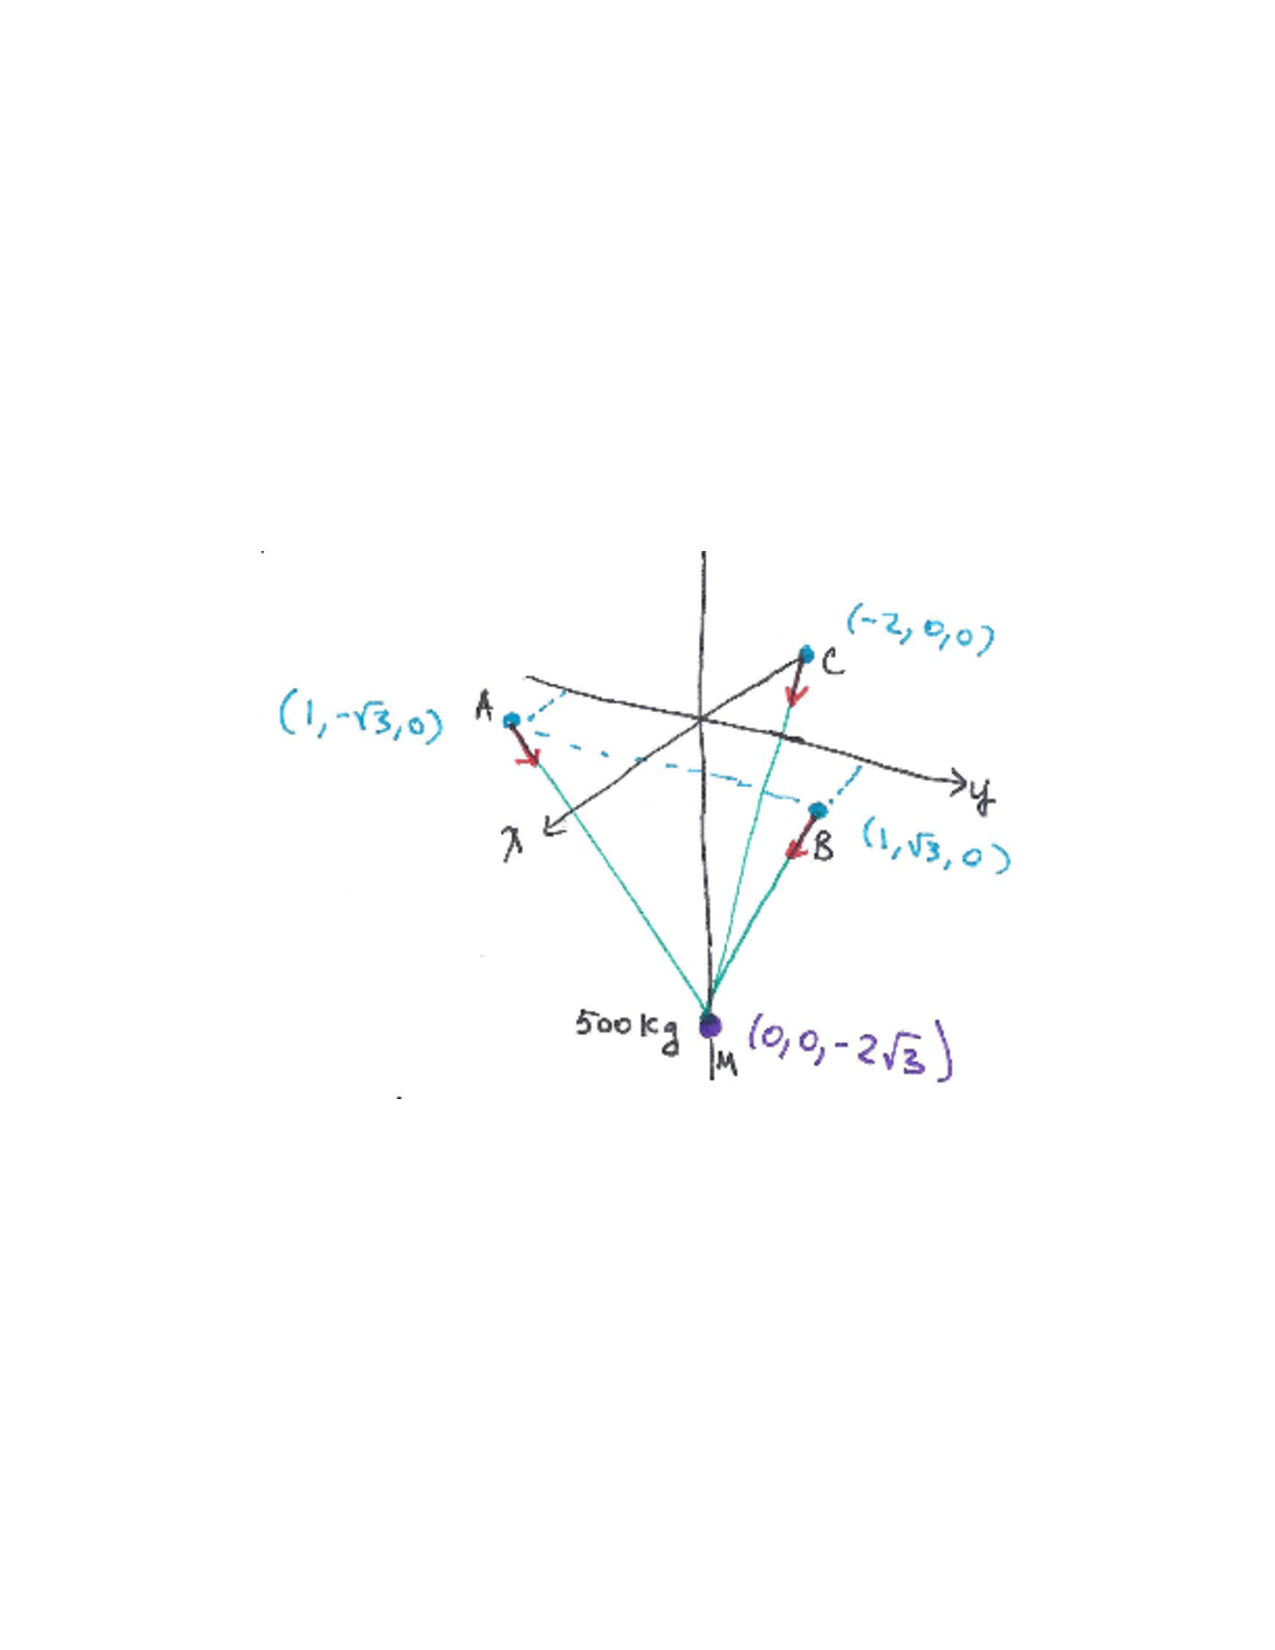
\includegraphics[trim= 230 270 170 270, scale=0.8]{Figure12-2-1.pdf}
%		\end{image}
%		
%	Notice that
%		\[
%		| \vec{a} | = | \vec{b} | = | \vec{c} | = 4
%		\]
%	and so unit vectors in the directions of $\vec{a}$, $\vec{b}$, and $\vec{c}$ are
%		\begin{align*}
%		&\vec{u}_a = \frac{1}{4} \langle -1, \sqrt{3}, -2\sqrt{3} \rangle  \\
%		&\vec{u}_b = \frac{1}{4} \langle -1, - \sqrt{3}, -2\sqrt{3} \rangle  \\
%		&\vec{u}_c = \frac{1}{4} \langle 2, 0, -2\sqrt{3} \rangle  .
%		\end{align*}
%		
%	The force on $M$ due to gravity is 
%		\[
%		\langle 0,0, -500 g \rangle
%		\]
%	where $g$ is the gravitational constant.  
%	We need to find real numbers $x$, $y$, and $z$ such that
%		\begin{align}
%		&-\frac{1}{4} x - \frac{1}{4} y + \frac{1}{2} z = 0    \qquad \Longrightarrow \qquad x+y-2z=0  \label{eqn1}  \\
%		&\frac{\sqrt{3}}{4} x - \frac{\sqrt{3}}{4} y + 0z = 0  \qquad \Longrightarrow \qquad x-y=0  \label{eqn2}  \\
%		&- \frac{\sqrt{3}}{2} x - \frac{\sqrt{3}}{2} y - \frac{\sqrt{3}}{2} z = -500g  \quad \Longrightarrow \quad x+y+z= \frac{1000g}{\sqrt{3}}. \label{eqn3}
%		\end{align}
%	By equation \eqref{eqn2} we have that $x=y$.  
%	Substituting this into equation \eqref{eqn1} we also see that $x=z$.  
%	So $x=y=z$.  
%	We plug this into equation \eqref{eqn3} to get that
%		\[
%		3x = \frac{1000g}{\sqrt{3}} \qquad \Longrightarrow \qquad x = \frac{1000g}{3\sqrt{3}}.
%		\]
%		
%	Thus,
%		\begin{itemize}
%		\item  The force along $AM$ is $\boxed{\frac{1000g}{3\sqrt{3}} \cdot \frac{1}{4} \langle -1, \sqrt{3},-2\sqrt{3} \rangle}$.
%		\item  The force along $BM$ is $\boxed{\frac{1000g}{3\sqrt{3}} \cdot \frac{1}{4} \langle -1, -\sqrt{3}, -2\sqrt{3} \rangle}$.
%		\item  The force along $CM$ is $\boxed{\frac{1000g}{3\sqrt{3}} \cdot \frac{1}{4} \langle 2,0,-2\sqrt{3} \rangle }$.
%		\end{itemize}
%	\end{freeResponse}
%		
%\end{problem}
%
%\begin{instructorNotes}
%Students need to take into account that the mass, and not the force, is given.  
%The students should also take advantage of the fact that the vectors are all of the same magnitude.  
%\end{instructorNotes}
%
%
%
%
%
%
%%problem 5
%\begin{problem}
%Find the work done by a constant force of $10 \hat{\imath} + 18 \hat{\jmath} - 6\hat{k}$ that moves an object up a ramp from $(2,3,7)$ to $(4,9,15)$.  
%Assume that distance is in feet and force in pounds.  
%Also, find the angle between the force and the ramp.
%	\begin{freeResponse}
%	First, let $\vec{F} = \langle 10,18,-7 \rangle$.  
%	Also, the vector from $(2,3,7)$ to $(4,9,15)$ is $\langle 2,6,8 \rangle$.  
%	Let $\vec{d} = \langle 2,6,8 \rangle$.  
%	Then the work done by the force is
%		\[
%		\vec{F} \cdot \vec{d} = 10 \cdot 2 + 18 \cdot 6 - 6 \cdot 8 = \boxed{80 \, ft \cdot lb}.
%		\]
%		
%	To calculate the angle, we compute
%		\[
%		\cos \theta = \frac{\vec{F} \cdot \vec{d}}{| \vec{F} | | \vec{d} |} = \frac{80}{\sqrt{460}\sqrt{104}}.
%		\]
%	and so
%		\[
%		\theta = \boxed{\cos^{-1} \left(  \frac{80}{\sqrt{460}\sqrt{104}} \right) \approx 1.196 \text{ radians}}
%		\]
%	\end{freeResponse}
%		
%\end{problem}
%
%\begin{instructorNotes}
%Simple work question.
%\end{instructorNotes}
%
%
%
%problem 6

\section{Challenge Problem}
%problem 8
\begin{problem}
Suppose that the deli at the Tiny Sparrow grocery store sells roast beef for $ \$ 9$ per pound, turkey for $ \$ 4$ per pound, salami for $\$ 5$ per pound, and ham for $\$ 7$ per pound.  
For lunches this week, Sam the sandwhich maker buys $1.5$ pounds of roast beef, $2$ pounds of turkey, no salami, and half a pound of ham.  
How can you use a dot product to compute Sam's total bill from the deli?
	\begin{freeResponse}
	The cost vector is
		\[
		\vec{c} = \langle 9,4,5,7 \rangle.
		\]
	The vector for Sam's order is
		\[
		\vec{o} = \left\langle \frac{3}{2}, 2, 0, \frac{1}{2} \right\rangle.
		\]
	Then Sam's bill is
		\[
		\vec{c} \cdot \vec{o} = 9(1.5) + 4(2) + 5(0) + 7(0.5) = 13.5 + 8 + 0 + 3.5 = \boxed{25}.
		\]
	\end{freeResponse}
	
\end{problem}

\begin{instructorNotes}

\end{instructorNotes}






	
	
	
	
	
	
	
	
	

	










								
				
				
	














\end{document} 


















